\chapter{HMD}
		\paragraph{} 
Uma parte significativa dos softwares de realidade aumenta requerem um uso de HMDs e a sua evolução está diretamente relacionada com a evolução da realidade virtual.\paragraph{}
 Mas o que é um HMD? \paragraph*{}
 HMD é um aparelho usado na cabeça, cujo objetivo é transmitir informação de forma visual através de um ecrã posicionado em frente a um ou ambos os olhos.O primeiro foi inventado por Morton Heilig(também inventor do Sensorama), e consistia num capacete com um ecrã que reproduzia um filme com uma visão estereoscópica em 3D , no entanto não inclua qualquer tipo de sensor de movimento ou interação com o usuário. 
 \begin{figure}
 \center
 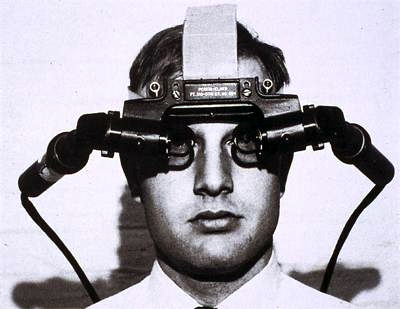
\includegraphics[scale=0.5]{imagens/HMD.jpg}
 \caption{Primeiro HMD, também conhecido como Sword of Damocles. \cite{3}}
 \end{figure}
\thispagestyle{empty}




